\documentclass[12pt, a4paper]{article}

\usepackage[utf8]{inputenc}
\usepackage[framemethod=TikZ]{mdframed}
\usepackage[hidelinks]{hyperref}
\usepackage{mathtools, amssymb, amsmath, cleveref, fancyhdr, geometry, tcolorbox, graphicx, float, subfigure, arydshln, url, setspace, framed, pifont, physics, ntheorem, utopia}

%%% for coding %%%
\usepackage{listings}
\usepackage[ruled, vlined, linesnumbered]{algorithm2e}

\geometry{a4paper, left=2cm, right=2cm, bottom=2cm, top=2cm}

\pagestyle{fancy}
\fancyhead{}
\fancyhead[L]{\leftmark}
\fancyhead[R]{\rightmark}
\fancyfoot{}
\fancyfoot[C]{\thepage}
%\renewcommand{\headrulewidth}{0pt}
\renewcommand{\footrulewidth}{0pt}

\hypersetup{
	colorlinks = true,
	bookmarks = true,
	bookmarksnumbered = true,
	pdfborder = 001,
	linkcolor = blue
}


\newcounter{index}[subsection]
\setcounter{index}{0}
\newenvironment*{df}[1]{\par\noindent\textbf{Definition \thesubsection.\stepcounter{index}\theindex\ (#1).}}{\par}

\newenvironment*{eg}{\begin{framed}\par\noindent\textbf{Example \thesubsection.\stepcounter{index}\theindex}}{\par\end{framed}}

\newenvironment*{thm}[1]{\begin{tcolorbox}\par\noindent\textbf{Theorem \thesubsection.\stepcounter{index}\theindex\ #1} \par}{\par\end{tcolorbox}}

\newenvironment*{cor}[1]{\par\noindent\textbf{Corollary \thesubsection.\stepcounter{index}\theindex\ #1}}{\par}
\newenvironment*{lem}[1]{\par\noindent\textbf{Lemma \thesubsection.\stepcounter{index}\theindex\ #1}}{\par}
\newenvironment*{ax}[1]{\par\noindent\textbf{Axiom \thesubsection.\stepcounter{index}\theindex\ #1}}{\par}
\newenvironment*{prop}[1]{\par\noindent\textbf{Proposition \thesubsection.\stepcounter{index}\theindex\ #1}}{\par}
\newenvironment*{conj}[1]{\par\noindent\textbf{Conjecture \thesubsection.\stepcounter{index}\theindex\ #1}}{\par}
\newenvironment*{nota}{\par\noindent\textbf{Notation \thesubsection.\stepcounter{index}\theindex.}}{\par}

\newcounter{nprf}[subsection]
\setcounter{nprf}{0}
\newenvironment*{prf}{\par\indent\textbf{\textit{Proof \stepcounter{nprf}\thenprf.}}}{\hfill$\blacksquare$\par}
\newenvironment*{dis}{\par\indent\textbf{\textit{Disproof \stepcounter{nprf}\thenprf.}}}{\hfill$\blacksquare$\par}
\newenvironment*{sol}{\par\indent\textbf{\textit{Solution \stepcounter{nprf}\thenprf.}}\par}{\hfill{$\square$}\par}

\newtheorem*{hint}{Hint.}
\newtheorem*{rmk}{Remark.}
\newtheorem*{ext}{Extension.}

\linespread{1.25}

\title{Emory University\\\textbf{MATH 361 Mathematical Statistics I}\\ Learning Notes}
\author{Jiuru Lyu}
\date{\today}

\def\Z{\mathbb{Z}}
\def\R{\mathbb{R}}
\def\C{\mathbb{C}}
\def\Q{\mathbb{Q}}
\def\E{\mathbb{E}}
\def\N{\mathbb{N}}
\def\d{\mathrm{d}}
\def\i{\mathrm{i}}
\def\Arg{{\mathrm{Arg}}}
\def\cis{\mathrm{cis}}
\def\epsilon{\varepsilon}
\def\emptyset{\varnothing}
\def\dsst{\displaystyle}

\begin{document}
\maketitle

\tableofcontents

\newpage
\section{Prerequisites}
\begin{df}{Geometric Series}
	A geometric series has the form \[\sum_{n=1}^\infty ar^{n-1}=a+ar+ar^2+\cdots\] If $\qty|r|<1$, then the series converges to $\dfrac{a}{1-r}$. Otherwise, it diverges. 	
\end{df}
\begin{eg}
	Does the series $\dsst\sum_{n=1}^\infty2^{2n}3^{1-n}$ converge or divers?
	\begin{sol}
		Note that \[2^{2n}3^{1-n}=\qty(2^2)^n3^{1-n}=4^n\qty(\dfrac{1}{3})^{n-1}=4\cdot4^{n -1}\qty(\dfrac{1}{3})^{n-1}=4\qty(\dfrac{4}{3})^{n-1}.\] So, \[\sum_{n=1}^\infty2^{2n}3^{1-n}=\sum_{n=1}^\infty4\qty(\dfrac{4}{3})^{n-1}\] is a geometric series, with $a=4$ and $r=\dfrac{4}{3}$.\par Since $\qty|r|=\qty|\dfrac{4}{3}|=\dfrac{4}{3}>1$, the series diverges.
	\end{sol}
\end{eg}
\begin{df}{Taylor Series}
	The Taylor series expanded about $a$ of a differentiable function $f$ is \[f(x)=\sum_{n=0}^\infty\dfrac{f^{(n)}(a)}{n!}(x-a)^n=f(a)+f'(a)(x-a)+\dfrac{f''(a)}{2!}(x-a)^2+\cdots.\]	
\end{df}
\begin{df}{Maclaurin Series}
	The Taylor series expanded about $a=0$.	
\end{df}
\begin{rmk}
	The Maclurin Series of $e^x$ is given by $e^x=\dsst\sum_{n=0}^\infty\dfrac{x^n}{n!}$.	
\end{rmk}
\begin{thm}{Binomial Expansion}
	\[(x+y)^n=\sum_{k=0}^n\binom{n}{k}x^ky^{n-k},\] where $\dsst\binom{n}{k}$ is read as ``$n$ choose $k$'' and can also be written as $nCk$. \[\binom{n}{k}=\dfrac{n!}{k!(n-k)!}=\dfrac{n(n-1)\cdots(n-k+1)}{k!}.\]
\end{thm}
\begin{thm}{Integration by Parts}
	\[\int u\ \d v=uv-\int v\ \d u.\]	
\end{thm}
\begin{eg}
	Evaluate $\dsst\int xe^{-x}\ \d x$.
	\begin{sol}
		Let $u=x,\ \d v=e^{-x}\ \d x$. So, $\d u=\d x$ and $v=\dsst\int e^{-x}\ \d x=-e^{-x}$. Then, \[\int xe^{-x}\ \d x=-xe^{-x}-\int-e^{-x}\ \d x=-xe^{-x}-e^{-x}+C.\]
	\end{sol}
\end{eg}
\begin{df}{Type I Improper Integral}
	If $\dsst\int_a^tf(x)\ \d x$ exists for all $t>0$, then \[\int_a^\infty f(x)\ \d x=\lim_{t\to\infty}\int_a^tf(x)\ \d x.\]
\end{df}
\begin{eg}
	Evaluate $\dsst\int_0^\infty xe^{-x}\ \d x$.
	\begin{sol}
		\[\begin{aligned}\int_0^\infty xe^{-x}\ \d x=\lim_{t\to\infty}\int_0^txe^{-x}\ \d x&=\lim_{t\to\infty}\qty\Big[-xe^{-x}-e^{-x}]_0^t\\&=\lim_{t\to\infty}\qty\Big(-te^{-t}-e^{-t}+1)\\&=-\lim_{t\to\infty}\qty(\dfrac{t}{e^t})-\lim_{t\to\infty}e^{-t}+1\\&=-\lim_{t\to\infty}\qty(\dfrac{1}{e^t})-0+1=-0-0+1=1.\end{aligned}\]
	\end{sol}
\end{eg}
\begin{eg}
	 Double Integrals over Irregular Domains.\\ Consider \[\dsst\iint_D4xy-y^4\ \d A,\] where $D$ is the region bounded between $y=\sqrt{x}$ and $y=x^3$. \par Evaluate this double integral over $D$.
	 \begin{sol}
	 	Firstly, we draw the diagram representing $D$ as follows: 
	 	\begin{center}
	 		\tikzset{every picture/.style={line width=0.75pt}}
	 		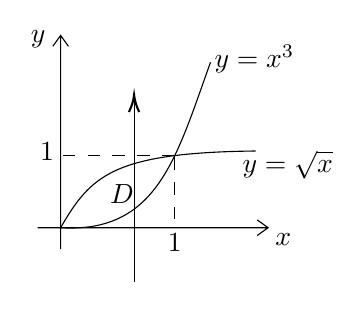
\begin{tikzpicture}[x=0.75pt,y=0.75pt,yscale=-.75,xscale=.75]
	 		\draw  (50,177.55) -- (198.1,177.55)(64.81,54) -- (64.81,191.27) (191.1,172.55) -- (198.1,177.55) -- (191.1,182.55) (59.81,61) -- (64.81,54) -- (69.81,61)  ;
	 		\draw    (64.81,177.55) .. controls (84.1,144.27) and (98.1,129.27) .. (190.1,128.27) ;
	 		\draw    (64.81,177.55) .. controls (127.1,181.27) and (139.1,132.27) .. (161.1,71.27) ;
	 		\draw    (112,212.27) -- (112,94.27) ;
	 		\draw [shift={(112,92.27)}, rotate = 90] [color={rgb, 255:red, 0; green, 0; blue, 0 }  ][line width=0.75]    (10.93,-3.29) .. controls (6.95,-1.4) and (3.31,-0.3) .. (0,0) .. controls (3.31,0.3) and (6.95,1.4) .. (10.93,3.29)   ;
	 		\draw  [dash pattern={on 4.5pt off 4.5pt}]  (138.1,132.27) -- (138.1,177.27) ;
	 		\draw  [dash pattern={on 4.5pt off 4.5pt}]  (138.1,131.27) -- (64.1,131.27) ;
	 		\draw (201,179.4) node [anchor=north west][inner sep=0.75pt]    {$x$};
	 		\draw (44,49.4) node [anchor=north west][inner sep=0.75pt]    {$y$};
	 		\draw (95,148.4) node [anchor=north west][inner sep=0.75pt]    {$D$};
	 		\draw (180,126.4) node [anchor=north west][inner sep=0.75pt]    {$y=\sqrt{x}$};
	 		\draw (162,58.4) node [anchor=north west][inner sep=0.75pt]    {$y=x^{3}$};
	 		\draw (132,179.4) node [anchor=north west][inner sep=0.75pt]    {$1$};
	 		\draw (50,121.4) node [anchor=north west][inner sep=0.75pt]    {$1$};
	 		\end{tikzpicture}
	 	\end{center}
	 	\[\begin{aligned}\iint_D4xy-y^3\ \d A=\int_0^1\int_{x^3}^{\sqrt{x}}4xy-y^3\ \d y\d x&=\int_0^1\qty[2xy^2-\dfrac{1}{4}y^4]_{x^3}^{\sqrt{x}}\ \d x\\&=\int_0^12x\qty(x-x^6)-\dfrac{1}{4}\qty(x^2-x^{12})\ \d x\\&=\int_0^12x^2-2x^7-\dfrac{1}{4}x^2+\dfrac{1}{4}x^{12}\ \d x\\&=\qty[\dfrac{2}{3}x^3-\dfrac{1}{4}x^8-\dfrac{1}{12}x^3+\dfrac{1}{52}x^{13}]_0^1\\&=\dfrac{2}{3}-\dfrac{1}{4}-\dfrac{1}{12}+\dfrac{1}{52}=\dfrac{55}{156}.\end{aligned}\]
	 \end{sol}
\end{eg}

\newpage
\section{Probability}
\subsection{Sample Space and Probability}
\begin{df}{Experiment}
	An \textit{experiment} is a procedure with well-defined outcome.	
\end{df}
\begin{df}{Sample Space/$S$}
	The \textit{sample space}, denoted as $S$ is the set of all possible outcomes of an experiment. 
\end{df}
\begin{df}{Event}
	An \textit{event} is a collection of outcomes.	
\end{df}
\begin{eg}
	Consider flipping two coins. Use $H$ to represent heads and $T$ to represent tails. Then, $S=\qty{HH, HT, TH, TT}$. Event ``one heads''$=\qty{HT, TH}$, and the event ``at least one heads''$=\qty{HT, TH, HH}$.
\end{eg}
\begin{df}{Union/$\cup$}
	$A\cup B$ is the \textit{union} of $A$ and $B$, meaning everything in $A$ and everything in $B$.
\end{df}
\begin{center}
\tikzset{every picture/.style={line width=0.75pt}}
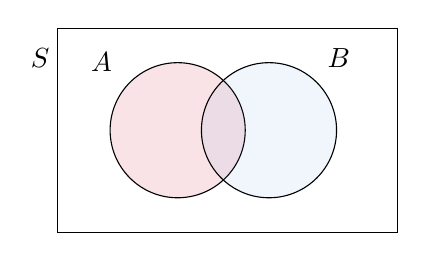
\begin{tikzpicture}[x=0.75pt,y=0.75pt,yscale=-1,xscale=1]
\draw   (111.1,128) -- (275.1,128) -- (275.1,226.27) -- (111.1,226.27) -- cycle ;
\draw  [fill={rgb, 255:red, 208; green, 2; blue, 27 }  ,fill opacity=0.11 ] (136.45,177.14) .. controls (136.45,159.16) and (151.02,144.59) .. (169,144.59) .. controls (186.98,144.59) and (201.55,159.16) .. (201.55,177.14) .. controls (201.55,195.11) and (186.98,209.68) .. (169,209.68) .. controls (151.02,209.68) and (136.45,195.11) .. (136.45,177.14) -- cycle ;
\draw  [fill={rgb, 255:red, 74; green, 144; blue, 226 }  ,fill opacity=0.08 ] (180.45,177.14) .. controls (180.45,159.16) and (195.02,144.59) .. (213,144.59) .. controls (230.98,144.59) and (245.55,159.16) .. (245.55,177.14) .. controls (245.55,195.11) and (230.98,209.68) .. (213,209.68) .. controls (195.02,209.68) and (180.45,195.11) .. (180.45,177.14) -- cycle ;
\draw (126,138.4) node [anchor=north west][inner sep=0.75pt]    {$A$};
\draw (240,136.4) node [anchor=north west][inner sep=0.75pt]    {$B$};
\draw (97,136.4) node [anchor=north west][inner sep=0.75pt]    {$S$};
\end{tikzpicture}	
\end{center}
\begin{df}{Intersection/$\cap$}
	$A\cap B$ is the \textit{intersection} of $A$ and $B$, everything in both $A$ and $B$	
\end{df}
\begin{center}
\tikzset{every picture/.style={line width=0.75pt}}
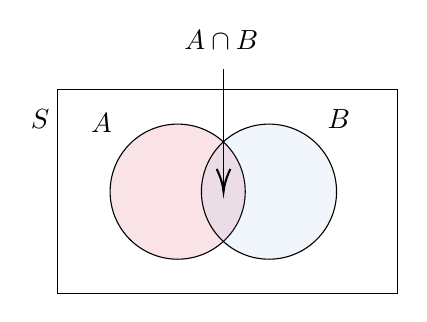
\begin{tikzpicture}[x=0.75pt,y=0.75pt,yscale=-1,xscale=1]
\draw   (111.1,128) -- (275.1,128) -- (275.1,226.27) -- (111.1,226.27) -- cycle ;
\draw  [fill={rgb, 255:red, 208; green, 2; blue, 27 }  ,fill opacity=0.11 ] (136.45,177.14) .. controls (136.45,159.16) and (151.02,144.59) .. (169,144.59) .. controls (186.98,144.59) and (201.55,159.16) .. (201.55,177.14) .. controls (201.55,195.11) and (186.98,209.68) .. (169,209.68) .. controls (151.02,209.68) and (136.45,195.11) .. (136.45,177.14) -- cycle ;
\draw  [fill={rgb, 255:red, 74; green, 144; blue, 226 }  ,fill opacity=0.08 ] (180.45,177.14) .. controls (180.45,159.16) and (195.02,144.59) .. (213,144.59) .. controls (230.98,144.59) and (245.55,159.16) .. (245.55,177.14) .. controls (245.55,195.11) and (230.98,209.68) .. (213,209.68) .. controls (195.02,209.68) and (180.45,195.11) .. (180.45,177.14) -- cycle ;
\draw    (191.1,118.27) -- (191.1,175.14) ;
\draw [shift={(191.1,177.14)}, rotate = 270] [color={rgb, 255:red, 0; green, 0; blue, 0 }  ][line width=0.75]    (10.93,-3.29) .. controls (6.95,-1.4) and (3.31,-0.3) .. (0,0) .. controls (3.31,0.3) and (6.95,1.4) .. (10.93,3.29)   ;
\draw (126,138.4) node [anchor=north west][inner sep=0.75pt]    {$A$};
\draw (240,136.4) node [anchor=north west][inner sep=0.75pt]    {$B$};
\draw (97,136.4) node [anchor=north west][inner sep=0.75pt]    {$S$};
\draw (171,98.4) node [anchor=north west][inner sep=0.75pt]    {$A\cap B$};
\end{tikzpicture}
\end{center}
\begin{df}{Complement/$A^c$}
	$A^c$ denotes the \textit{complement} of $A$, meaning everything in$S$ that is not in $A$.	
\end{df}
\begin{center}
\tikzset{every picture/.style={line width=0.75pt}}
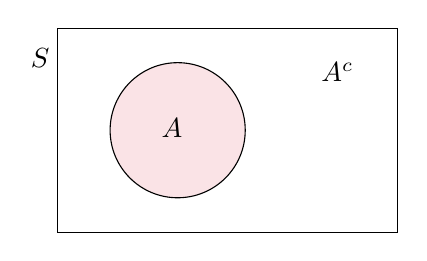
\begin{tikzpicture}[x=0.75pt,y=0.75pt,yscale=-1,xscale=1]
\draw   (111.1,128) -- (275.1,128) -- (275.1,226.27) -- (111.1,226.27) -- cycle ;
\draw  [fill={rgb, 255:red, 208; green, 2; blue, 27 }  ,fill opacity=0.11 ] (136.45,177.14) .. controls (136.45,159.16) and (151.02,144.59) .. (169,144.59) .. controls (186.98,144.59) and (201.55,159.16) .. (201.55,177.14) .. controls (201.55,195.11) and (186.98,209.68) .. (169,209.68) .. controls (151.02,209.68) and (136.45,195.11) .. (136.45,177.14) -- cycle ;
\draw (160,170.4) node [anchor=north west][inner sep=0.75pt]    {$A$};
\draw (97,136.4) node [anchor=north west][inner sep=0.75pt]    {$S$};
\draw (237,143.4) node [anchor=north west][inner sep=0.75pt]    {$A^{c}$};
\end{tikzpicture}	
\end{center}
\begin{cor}{}
	$A\cap A^c=\qty{}=\emptyset$.	
\end{cor}
\begin{df}{Mutually Exclusive}
	Two sets $A$ and $B$ over the same sample space are \textit{mutually exclusive} if they have no outcomes in common. i.e., $A\cap B=\emptyset$.	
\end{df}
\begin{rmk}
	$A$ and $A^c$ are mutually exclusive, but not all sets mutually exclusive are complements of each other.	
\end{rmk}
\begin{df}{Probability Function}
	Let $A$ be an event over a sample space $S$. Then, $P(A)$ denotes the \textit{probability} of $A$ and $P$ is the \textit{probability function}. The probability function $P$ assigns a number $P(A)$ for each event $A\subseteq S$.
\end{df}
\begin{ax}{Kolmogorov Axioms}
	\begin{enumerate}
		\item Let $A$ be an event in $S$, then $P(A)\geq0$.
		\item $P(S)=1$.
		\item If $A$ and $B$ are mutually exclusive, then $P(A\cup B)=P(A)+P(B)$.
		\item If $A_1,\dots,A_n,\dots$ are mutually exclusive sets, then \[P\qty(\bigcup_{i=1}^\infty A_i)=\sum_{i=1}^\infty P(A_i).\]
	\end{enumerate}	
\end{ax}
\begin{prop}{}
	$P(A^c)=1-P(A)$.	
\end{prop}
\begin{prf}
	Note that $P(S)=1$. Since $A^c\cup A=S$, we have $P(A\cap A^c)=1$. Since $A$ and $A^c$ are mutually exclusive, $P(A\cup A^c)=P(A)+P(A^c)=1$. So, $P(A^c)=1-P(A)$.	
\end{prf}
\begin{prop}{}
	$P(\emptyset)=0$.	
\end{prop}
\begin{prf}
	Note that $P(S)=1$. Then, $P(S^c)=1-P(S)$. By definition, we know $S^c=\emptyset$. So, $P(\emptyset)=1-P(S)=1-1=0$.	
\end{prf}
\begin{prop}{}
	$P(A\cup B)=P(A)+P(B)-P(A\cap B)$	
\end{prop}
\begin{prf}
	Consider the following Venn diagram: 
	\begin{center}
	\tikzset{every picture/.style={line width=0.75pt}}
	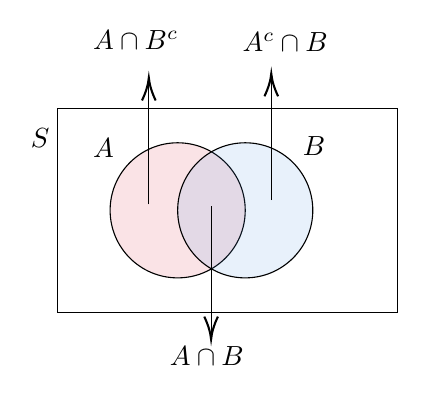
\begin{tikzpicture}[x=0.75pt,y=0.75pt,yscale=-1,xscale=1]
	\draw   (111.1,128) -- (275.1,128) -- (275.1,226.27) -- (111.1,226.27) -- cycle ;
	\draw  [fill={rgb, 255:red, 208; green, 2; blue, 27 }  ,fill opacity=0.11 ] (136.45,177.14) .. controls (136.45,159.16) and (151.02,144.59) .. (169,144.59) .. controls (186.98,144.59) and (201.55,159.16) .. (201.55,177.14) .. controls (201.55,195.11) and (186.98,209.68) .. (169,209.68) .. controls (151.02,209.68) and (136.45,195.11) .. (136.45,177.14) -- cycle ;
	\draw  [fill={rgb, 255:red, 74; green, 144; blue, 226 }  ,fill opacity=0.13 ] (169,177.14) .. controls (169,159.16) and (183.57,144.59) .. (201.55,144.59) .. controls (219.52,144.59) and (234.1,159.16) .. (234.1,177.14) .. controls (234.1,195.11) and (219.52,209.68) .. (201.55,209.68) .. controls (183.57,209.68) and (169,195.11) .. (169,177.14) -- cycle ;
	\draw    (185.1,175.27) -- (185.1,237.27) ;
	\draw [shift={(185.1,239.27)}, rotate = 270] [color={rgb, 255:red, 0; green, 0; blue, 0 }  ][line width=0.75]    (10.93,-3.29) .. controls (6.95,-1.4) and (3.31,-0.3) .. (0,0) .. controls (3.31,0.3) and (6.95,1.4) .. (10.93,3.29)   ;
	\draw    (155.1,174.27) -- (155.1,115.27) ;
	\draw [shift={(155.1,113.27)}, rotate = 90] [color={rgb, 255:red, 0; green, 0; blue, 0 }  ][line width=0.75]    (10.93,-3.29) .. controls (6.95,-1.4) and (3.31,-0.3) .. (0,0) .. controls (3.31,0.3) and (6.95,1.4) .. (10.93,3.29)   ;
	\draw    (214.1,172.27) -- (214.1,113.27) ;
	\draw [shift={(214.1,111.27)}, rotate = 90] [color={rgb, 255:red, 0; green, 0; blue, 0 }  ][line width=0.75]    (10.93,-3.29) .. controls (6.95,-1.4) and (3.31,-0.3) .. (0,0) .. controls (3.31,0.3) and (6.95,1.4) .. (10.93,3.29)   ;
	\draw (127,141.4) node [anchor=north west][inner sep=0.75pt]    {$A$};
	\draw (97,136.4) node [anchor=north west][inner sep=0.75pt]    {$S$};
	\draw (228,140.4) node [anchor=north west][inner sep=0.75pt]    {$B$};
	\draw (127,89.4) node [anchor=north west][inner sep=0.75pt]    {$A\cap B^{c}$};
	\draw (199,90.4) node [anchor=north west][inner sep=0.75pt]    {$A^{c} \cap B$};
	\draw (164,241.4) node [anchor=north west][inner sep=0.75pt]    {$A \cap B$};
	\end{tikzpicture}
	\end{center}
	Note that $P(A)=P(A\cap B)+P(A\cap B^c)$ and $P(B)=P(A\cap B)+P(A^c\cap B)$. So, we have \begin{equation}\label{eq1}P(A)+P(B)=\boxed{P(A\cap B^c)+P(A^c\cap B)+P(A\cap B)}+P(A\cap B).\end{equation} From the Venn diagram, we notice that $P(A\cap B^c)+P(A^c\cap B)+P(A\cap B)$ is exactly $P(A\cup B)$. So, Eq. (\ref{eq1}) becomes $P(A)+P(B)=P(A\cup B)+P(A\cap B)$. That is exactly what is required: $P(A\cup B)=P(A)+P(B)-P(A\cap B)$.
\end{prf}
\begin{df}{Classical Probability}
	In a discrete and finite case, $S$ is finite and all outcomes are equally likely, and the probability function is defined as \[P(A)=\dfrac{\qty|A|}{\qty|S|},\] where $\qty|A|$ is the cardinality of $A$ and $\qty|S|$ is the cardinality of $S$.	
\end{df}
\begin{eg}
	Despite the definition of classical probability (probability function defined for a discrete and finite case), there are other definitions of probability functions: 
	\begin{enumerate}
		\item Discrete and Countably Infinite: \par Let $S=\N$ be the set of natural numbers. Then, \[P(k)=\dfrac{1}{2^k}.\] It can also be verified that \[P(S)=\sum_{k=1}^\infty\dfrac{1}{2^k}=1.\]
		\item Continuous and Uncountably Infinite: \par Let $S=\qty[0,1]$. Suppose $E$ is a subset of $\qty[0,1]$ such that $\dsst\int_E\ \d x$ is defined. Then, \[P(E)=\int_E\ \d x,\] and it can also be verified that $P(S)=1$.
	\end{enumerate}	
\end{eg}

\newpage
\subsection{Conditional Probability and Independence}
\begin{df}{Conditional Probability}
	We read $P(A|B)$ as the probability of $A$ given $B$. Knowing $B$ occurs, we create a new sample space, in which the probability of $A$ occurs changes: \[P(A|B)=\dfrac{\qty|A\cap B|}{\qty|B|}=\dfrac{\qty|A\cap B|}{\qty|B|}\cdot\dfrac{1/\qty|S|}{1/\qty|S|}=\dfrac{\qty|A\cap B|/\qty|S|}{\qty|B|/\qty|S|}=\dfrac{P(A\cap B)}{P(B)}.\]	
\end{df}
\begin{cor}{}
	$P(A\cap B)=P(A|B)P(B)$
\end{cor}
\begin{eg}
	Find the probability of dealing $A$ first, $2$ second, and $3$ third.
	\begin{sol}
		\[\begin{aligned}P(\text{dealing }A,2,3)&=P(A\text{ first})P(2\text{ second}|A\text{ first})P(3\text{ third}|A\text{ first}\cap2\text{ second})\\&=\dfrac{4}{52}\cdot\dfrac{4}{51}\cdot\dfrac{4}{50}\end{aligned}\]
	\end{sol}
\end{eg}
\begin{cor}{}
	$P(A_1\cap A_2\cap A_3)=P(A_1)P(A_2|A_1)P(A_3|A_2\cap A_1).$	
\end{cor}
\begin{thm}{The Law of Total Probability}
	Suppose the sample space $S=A_1\cup A_2\cup\cdots\cup A_n$, with $A_i\cap A_j=\emptyset\quad\forall i\neq j$	. Then, \[P(B)=P(B\cap A_1)+P(B\cap A_2)+\cdots+P(B\cap A_n).\]
\end{thm}
\begin{rmk}
	This theorem gives us a nice way to partition the sample space. 	
\end{rmk}
\begin{eg}
	\begin{center}
	\tikzset{every picture/.style={line width=0.75pt}}
	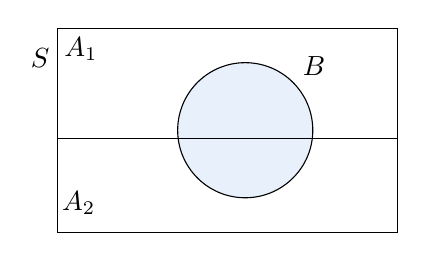
\begin{tikzpicture}[x=0.75pt,y=0.75pt,yscale=-1,xscale=1]
	\draw   (111.1,128) -- (275.1,128) -- (275.1,226.27) -- (111.1,226.27) -- cycle ;
	\draw  [fill={rgb, 255:red, 74; green, 144; blue, 226 }  ,fill opacity=0.13 ] (169,177.14) .. controls (169,159.16) and (183.57,144.59) .. (201.55,144.59) .. controls (219.52,144.59) and (234.1,159.16) .. (234.1,177.14) .. controls (234.1,195.11) and (219.52,209.68) .. (201.55,209.68) .. controls (183.57,209.68) and (169,195.11) .. (169,177.14) -- cycle ;
	\draw    (111,181) -- (275,181) ;
	\draw (113.1,131.4) node [anchor=north west][inner sep=0.75pt]    {$A_{1}$};
	\draw (97,136.4) node [anchor=north west][inner sep=0.75pt]    {$S$};
	\draw (228,140.4) node [anchor=north west][inner sep=0.75pt]    {$B$};
	\draw (112.1,205.4) node [anchor=north west][inner sep=0.75pt]    {$A_{2}$};
	\end{tikzpicture}
	\end{center}
	As represented in the diagram above, $P(B)=P(B\cap A_1)+P(B\cap A_2)$. 
\end{eg}
\begin{thm}{Bayes Theorem}
	\[P(B|A)=\dfrac{P(A\cap B)}{P(A)}=\dfrac{P(A|B)P(B)}{P(A|B)P(B)+P(A|B^c)P(B^c)}.\]	
\end{thm}
\begin{df}{Independence}
	Events $A$ and $B$ are \textit{independent} if $P(A|B)=P(A)$, meaning the occurrence of $B$ does note affect the occurrence of $A$.
\end{df}
\begin{cor}{}
	If $A$ and $B$ are independent, then $P(A\cap B)=P(A|B)P(B)=P(A)P(B).$
\end{cor}
\begin{eg}{Coronary Artery Disease (CAD)}
	\par The probability of someone having CAD is 60\%. In a study of 101 patients, 37 of them are known to NOT have CAD and 64 are known to have CAD. Of the 37 patients without CAD, 34 had negative tests while 3 had positive tests. Of the 64 with CAD, 54 had positive tests and 10 had negative tests. Find the probability of a patient has CAD given positive test.
	\begin{sol}
		Let $T+$ be positive test, $T-$ be negative test, $D+$ be presence of CAD, and $D-$ be absence of CAD. Then, from the problem, we have \[P(D+)=0.6;\quad P(D-)=1-P(D+)=0.4\] and \[P(T+|D+)=\dfrac{54}{64}\approx0.84;\quad P(T-|D-)=\dfrac{34}{37}\approx0.92;\quad P(T+|D-)=\dfrac{3}{37}\approx0.08.\] Then, by Bayes Theorem, \[\begin{aligned}P(D+|T+)&=\dfrac{P(T+|D+)P(D+)}{P(T+|D+)P(D+)+P(T+|D-)P(D-)}\\&=\dfrac{0.84\times0.6}{0.84\times0.6+0.08\times0.4}\approx\boxed{0.94}.\end{aligned}\]
	\end{sol}
\end{eg}



\end{document}